% TO DO:CHAPTER 4.3 and 4.4 (architecture and algorithms), CHAPTER 5, CONTRIBUTIONS, PLOTTING NOTES (TAYLOR), FINISH TEST WRITEUP
\documentclass[a4paper, oneside, 11pt]{report}
\usepackage{epsfig,pifont,float,multirow,amsmath,amssymb}
\usepackage{natbib}
\newcommand{\mc}{\multicolumn{1}{c|}}
\newcommand{\mb}{\mathbf}
\newcommand{\mi}{\mathit}
\newcommand{\oa}{\overrightarrow}
\newcommand{\bs}{\boldsymbol}
\newcommand{\ra}{\rightarrow}
\newcommand{\la}{\leftarrow}
\usepackage{algorithm}
\usepackage{algorithmic}
\topmargin = 0pt
\voffset = -80pt
\oddsidemargin = 15pt
\textwidth = 425pt
\textheight = 750pt

\begin{document}

    \begin{titlepage}
        \begin{center}
            \rule{12cm}{1mm} \\
            \vspace{1cm}
            {\large  CMP-6048A/7009A Advanced Programming} %Delete as appropriate
            \vspace{7.5cm}
            \\{\Large Project Report - 13 January 2025}
            \vspace{1.5cm}
            \\{\LARGE Maths Interpreter software} % You can add to this title of modify it if you wish
            \vspace{1.0cm}
            \\{\Large Group members: \\ Ethan Colman, Taylor Holton, Aaron Hurrell, Connor Stansfield.\ }
            \vspace{10.0cm}
            \\{\large School of Computing Sciences, University of East Anglia}
            \\ \rule{12cm}{0.5mm}
            \\ \hspace{8.5cm} {\large Version 2.0}
        \end{center}
    \end{titlepage}


    \setcounter{page}{1}
%\pagenumbering{roman}
%\newpage

% ============================================================== ABSTRACT ================================================================
    \begin{abstract}
        In the past 80 years the capacity of computer programs has soared. During this time programmers have moved from writing programs in pure machine code to various forms of assembly, up into increasingly higher-level programming languages. This shift in the way programmers interact with computers is owed in large part to the development of compilers and interpreters, which facilitate more powerful and human-readable code. In this report, we use a functional language, \verb|F#|, to develop a basic interpreter designed to handle mathematical computations as well as some basic language features such as iteration as well as variable or function binding. We outline our development process in terms of agile sprints completed to develop individual features or sets of features, and we discuss the final product in greater detail.

% Please replace this section with your own abstract. An abstract is a brief summary (maximum 250 words) of your entire project. It should cover your objectives, your methodologies used, a brief developmental history, your final results, in particular covering the optional tasks, and a discussion and conclusion. You do not cover the literature or background in an abstract nor should you use abbreviations or acronyms. The remainder of this report template has clear chapter titles and we suggest to stick to these although you can organise your material inside each chapter to your own preferences. A guideline in size is approximately 3,500 words (not including abstract, captions and references) but no real limit on figures, tables, diagrams, pseudo-code etc.
    \end{abstract}

% ============================================================== CHAPTER 1 ===============================================================
    \chapter{Introduction}
    \label{chap:intro}
    The introduction should be brief and comprise the following:

    \section{Project statement}
% \paragraph{}
% We will produce a mathematics package written using the .NET environment. We will use C# with Avalonia to produce an application with a graphical user interface, which includes a graph plotting utility as well as a mathematical interpreter capable of processing a wide range of common mathematical utilities.
% \paragraph{}
% Said interpreter will be written in F#, a functional language. The interpreter will deconstruct user input into a series of tokens, which are then processed by a parser to produce a result or create some binding such as a function or variable.
    \paragraph{}
    We will produce a mathematics package written using the .NET environment. We will produce an application with a graphical user interface, which includes a graph plotting utility as well as a mathematical interpreter capable of processing a wide range of common mathematical operations. The application will take user input, which is then lexed and parsed by the interpreter. The output will then be written to an output field while also being plotted to the graph window.

    \section{Aims and objectives}
    \paragraph{}
    We plan to:
    \begin{itemize}
        \item produce a basic mathematical interpreter
        \item produce a graphical user interface to output the results of said interpreter
        \item expand our implementation of the interpreter to cover complex features, such as complex numbers, function bindings with parameter passing and evaluating boolean expressions
        \item expand our user interface to support graph plotting and associated features.
    \end{itemize}
    \paragraph{}
    To be more specific about the requirements of our project, a table is included in Appendix \ref{MOSCOW} indicating the priority of different objectives by way of MoSCoW Requirements Analysis.

% \paragraph{}
% On top of this, we should aim to implement different representations of numbers, such as rational numbers which are more suitable for storing numbers when exact precision is required (which a floating point number cannot provide). We should also add further features, such as functions - sequences of tokens stored to be evaluated at the point of execution, complete with a parameter system to provide function-level scope to the expression. Features like this, in addition to the implementation of expression iteration (either in the GUI or interpreter) could be used to generate a series of coordinates for the graph plotting utility of the application.

% Clearly specify the main aim and objective(s) and subsequent tasks of your project. You can use a MoSCoW to further elaborate on each individual task. If you do so, use a table with three columns (e.g.\ Table \ref{Table1}), the first one having the four categories; the second column a brief description of the task and the third column further elaboration or comments on the task. Note that a MoSCoW is normally for functional requirements only. You should treat non-functional requirements in a separate MoSCoW.
% ============================================================== CHAPTER 2 ===============================================================
    \chapter{Background}

    When developing this project, we consulted and referenced some similar systems. These systems were Desmos \citep{Desmos:2023} Matlab \citep{Matlab:2023} and Wolfram Alpha \citep{Wolfram-Alpha:2025}. \\

    Focusing on Desmos first, this web application has a series of calculators available to users. The graphing calculator with its small input area and much larger plotting area is useful for graphs and lines. The scientific calculator has a large input area with buttons for functions, numbers, and other purposes. These are just two calculators available to users. Some of its capabilities include Interactive variables for graphs, various function graphing, and calculus with a limitation of limits. \\

    MatLab is a programming language that is used across data analysis, control systems, and robots. For these services, it has features such as; interactive apps, specialised libraries, and tools used for generating embedded code. It can do matrix manipulation \citep{Matlab-Feat:2025} and because of its large library of mathematical functions, it can also fulfil a role similar to our system or Desmos. \\

    Wolfram Alpha, similarly to Desmos, is also a web application with the capacity to solve mathematical problems inputted into it and graph lines. Unlike Desmos, Wolfram Alpha fulfils a purpose of answering questions across a much broader range from questions about maths to questions about nutritional content of food. Another difference is that rather than having a number of environments for the user, it has one with a text input. Then it will output the solution based on the input. For example, an input of "plot sin 30" will create a linear line of 0.5 on the y axis. (\ref{WolframPlotted})
    However, if you just enter "sin 30", you will not get a result formatted as a graph. (\ref{WolframUnplotted})
    Therefore its acts similarly to a search engine with a number of functions that you can call to alter its output format. \\

    Here is a feature comparison of the three systems. \\//////

    With an idea of what our system would do and potential ways to show it, we now needed an understanding of how we were going to do it.


    Also, cite the books \citep{Nystrom:2021} or documentation \citep{WPF:2023} that you consulted.
% ============================================================== CHAPTER 3 ===============================================================
    \chapter{Development History}\label{Chap:DevHist}
% Basic Implementation (INT1) & GUI (GUI1)
% Variable Assignment (INT2)
% Plotting (GUI2)
% Pi and Abs
% Static Type System
% Functions
% Booleans
% Count Controlled Loops
% Rationals
% Trigonometric and Natural Logarithm Functions

% Symbol Table as a Class, Embedded Type Checks

    \paragraph{Foreword} The presentation of the sprints below is as accurate as possible. However, most of these sprints have some level of overlap with others. This is because for each feature we would work individually on it and add it to the main git branch when it was complete. Additionally, small-scale commits for minor tweaks or bugfixes have been omitted, unless substantially relevant. Finally, for each sprint we reused the unit tests from previous sprints, adding new tests where appropriate. A full table of these tests can be found in the Appendix.


% ---------------------------------------------------------------- SPRINT 1 ----------------------------------------------------------------
    \section{Sprint 1: Basic Implementation and GUI}
    \subsection{Grammar in BNF}
    \begin{verbatim}
// <E>        ::= <T> <Eopt>
// <Eopt>     ::= "+" <T> <Eopt> | "-" <T> <Eopt> | <empty>
// <T>        ::= <F> <Topt>
// <Topt>     ::= "*" <F> <Topt> | "/" <F> <Topt> |  "%" <F> <Topt> |<empty>
// <F>        ::= <NR> <Fopt>
// <Fopt>     ::= "^" <NR> <Fopt> | "-" <NR> | "+" <NR> | <empty>
// <NR>       ::= "Int" <value> | "Flt" <value> | "(" <E> ")"
    \end{verbatim}

    \subsection{Basic GUI}
    We used Avalonia with C\# to develop a basic GUI - see Figure \ref{gui01}.

    \begin{figure}[htb]
        \begin{center}
% REPLACE IMAGE!!!!
            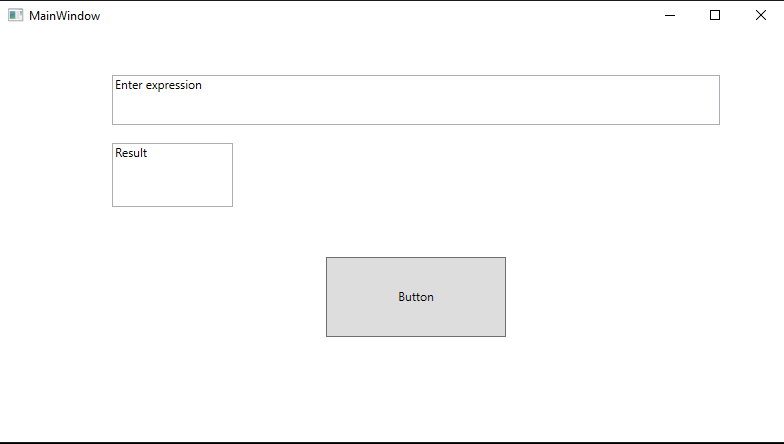
\includegraphics[width=0.9 \columnwidth]{GUI_01}
            \caption{GUI, first revision.}
            \label{gui01}
        \end{center}
    \end{figure}

    \subsection{Commentary}
    An additional pair of functions, F and Fopt, were added to the parser to offer an additional level of precedence.
    This allows the parser to evaluate the unary minus and power operators before the rest of the arithmetic operators.
    Which allows unary minus to be evaluated properly (as instead it would be evaluated as a binary minus and throw an error).


    \subsection{Testing}
    This build passed every test from our unit tests \ref{ArithTest}, except:

    \begin{center}
        \begin{tabular}{|p{1.5in}|p{1.5in}|p{1.6in}|p{1.6in}|p{2.4in}|}
            \hline
            TEST NAME & INPUT & EXPECTED & RESULT \\
            \hline
            T1.DivInt & "5 / 2" & 2 & 2.5 \\
            \hline
            T1.UnaryPlus & "+3 + 4" & 7 & Error \\
            \hline
        \end{tabular}
    \end{center}


    \clearpage
% ------------------------------------------------------------- END OF SPRINT ------------------------------------------------------------------
% ---------------------------------------------------------------- SPRINT 2 ----------------------------------------------------------------
    \section{Sprint 2: Variable Assignment}
    \subsection{Grammar in BNF}
    \begin{verbatim}
Grammar in BNF:
<E>        ::= <T> <Eopt>
<Eopt>     ::= "+" <T> <Eopt> | "-" <T> <Eopt> | <empty>
<T>        ::= <F> <Topt>
<Topt>     ::= "*" <F> <Topt> | "/" <F> <Topt> |  "%" <F> <Topt> |<empty>
<F>        ::= <NR> <Fopt>
<Fopt>     ::= "^" <NR> <Fopt> | "-" <NR> | <empty>
<NR>       ::= "Var" <value> "Assign" <NR> | "Var" <value> | "Int" <value> |                  "Flt" <value> | "(" <E> ")"

    \end{verbatim}

    \subsection{Commentary}
    In order to store variables we made use of a hash map for fast access to the variable associated with the requested binding. This table is the only mutable component of our software.

    The lexer reads any string of characters not beginning with a numeric character as a "Var". It parses the remaining characters until it finds white space to create a string associated with the "Var" terminal symbol.

    The parser then looks for the pattern "Var :: Assign :: tail" ("=" is lexed as Assign). It then calls NR on the tail, and adds the string associated with the "Var" symbol and the the result of "NR tail" to the symbol table as a key value pair.

    When the "Var :: tail" pattern if found, and the "Var :: Assign :: tail" pattern isn't, the program checks to see if the requested variable is in the symbol table. If it is, a number is returned; if it isn't, an exception is raised.

    \subsection{Testing}
    This build passed every test from our unit tests \ref{ArithTest} and \ref{VarAssignTest}, except:

    \begin{center}
        \begin{tabular}{|p{1.5in}|p{1.5in}|p{1.6in}|p{1.6in}|p{2.4in}|}
            \hline
            TEST NAME & INPUT & EXPECTED & RESULT \\
            \hline
            T1.DivInt & "5 / 2" & 2 & 2.5 \\
            \hline
            T1.UnaryPlus & "+3 + 4" & 7 & Error \\
            \hline
        \end{tabular}
    \end{center}


    \clearpage
% ------------------------------------------------------------- END OF SPRINT ------------------------------------------------------------------
% ---------------------------------------------------------------- SPRINT 3 ----------------------------------------------------------------
    \section{Sprint 3: Plotting}
    \subsection{Grammar in BNF}
    No change was made to the grammar at this stage, as plotting is not directly relevant to the interpreter.

    \subsection{Commentary}
    \{FOR TAYLOR TO WRITE\}

    \subsection{Testing}
    Please refer to this (\ref{PlotTest}) in the appendices to view our Testing. \\

    \clearpage
% ------------------------------------------------------------- END OF SPRINT ------------------------------------------------------------------

% ---------------------------------------------------------------- SPRINT 4 ----------------------------------------------------------------
    \section{Sprint 4: Pi and Abs}
    \subsection{Grammar in BNF}
    \begin{verbatim}
Grammar in BNF:

<E>        ::= <T> <Eopt>
<Eopt>     ::= "+" <T> <Eopt> | "-" <T> <Eopt> | <empty>
<T>        ::= <F> <Topt>
<Topt>     ::= "*" <F> <Topt> | "/" <F> <Topt> |  "%" <F> <Topt> |<empty>
<F>        ::= <NR> <Fopt>
<Fopt>     ::= "^" <NR> <Fopt> | "-" <NR> |<empty>
<NR>       ::=  "Var" <value> "Assign" <NR> | "Var" <value> |
                "Num Int" <value> | "Num Flt" <value> |
                "Pi" | "Abs" <NR> | "(" <E> ")"
    \end{verbatim}

    \subsection{Commentary}
    During this sprint we added a token that returns the value of Pi as a float, and the Abs function which returns the absolute value of a number.


    \subsection{Testing}
    ALL WORKS!!!


    \clearpage
% ------------------------------------------------------------- END OF SPRINT ------------------------------------------------------------------
% ---------------------------------------------------------------- SPRINT 5 ----------------------------------------------------------------
    \section{Sprint 5: Static Type System}
    \subsection{Grammar in BNF}
    \begin{verbatim}
Grammar in BNF:

<E>        ::= <T> <Eopt>
<Eopt>     ::= "+" <T> <Eopt> | "-" <T> <Eopt> | <empty>
<T>        ::= <F> <Topt>
<Topt>     ::= "*" <F> <Topt> | "/" <F> <Topt> |  "%" <F> <Topt> |<empty>
<F>        ::= <NR> <Fopt>
<Fopt>     ::= "^" <NR> <Fopt> | "-" <NR> |<empty>
<NR>       ::=  "Var" <value> "Assign" <NR> |
                "Typ Auto" "Var" <value> "Assign" <NR> |
                "Typ Integer" "Var" <value> "Assign" <NR> |
                "Typ Float" "Var" <value> "Assign" <NR> |
                "Var" <value> |
                "Num Int" <value> | "Num Flt" <value> |
                "Pi" | "Abs" <NR> |
                "(" <E> ")"
    \end{verbatim}
    \subsection{Commentary}
    Additional patterns are added for variable assignment such that users can either explicitly specify the type of variable assignment, or let the interpreter infer it.
    If one of the explicit assignments are used (such as "Typ Integer::Var::Assign::tail"), or a variables value is being reassigned, then the interpreter checks that the types match before assignment, throwing an error if they do not.

    Explicit type declarations are specified with the keywords: \verb|int, float, frac| and \verb|bool|.
    While inferred typing can be specified with the keyword \verb|var| in place of an explicit type.
    A legacy option for variable declaration also exists where type declaration is omitted.
    This is for use in sending plotting functions from the front end to the interpreter and could be removed in future if the plotting were rewritten.

    \subsection{Testing}
    ALL WORKS!!!


    \clearpage
% ------------------------------------------------------------- END OF SPRINT ------------------------------------------------------------------
% ---------------------------------------------------------------- SPRINT 6----------------------------------------------------------------
    \section{Sprint 6: Functions}
    \subsection{Grammar in BNF}
    \begin{verbatim}
Grammar in BNF:

<E>        ::= <T> <Eopt>
<Eopt>     ::= "+" <T> <Eopt> | "-" <T> <Eopt> | <empty>
<T>        ::= <F> <Topt>
<Topt>     ::= "*" <F> <Topt> | "/" <F> <Topt> |  "%" <F> <Topt> |<empty>
<F>        ::= <NR> <Fopt>
<Fopt>     ::= "^" <NR> <Fopt> | "-" <NR> |<empty>
<NR>       ::=  "Var" <value> "Assign" <NR> |
                "Typ Auto" "Var" <value> "Assign" <NR> |
                "Typ Integer" "Var" <value> "Assign" <NR> |
                "Typ Float" "Var" <value> "Assign" <NR> |
                "Fn" "Var" <value> "Assign" 0 |
                "Var" <value> |
                "Num Int" <value> | "Flt" <value> |
                "Pi" | "Abs" <NR> |
                "(" <E> ")"
    \end{verbatim}

    \subsection{Commentary}
    Here, we updated the symbol table to hold functions as well as variables. This is achieved by modifying the table to take a 3-tuple as a value - this tuple contains a BindingType (indicating if a binding is a Function or Variable), a list of parameters, and a list of tokens representing the function body. For variables, the parameter list is left intentionally blank when being assigned, and the token list is only one token long, holding a "Num".

    The "Fn" token is used in the assign pattern to specify that the binding is a function - the assignment code sets the BindingType to "Function" and parses a parameter sequence out of the left side of the assignment.

    When "Var::tail" is matched, the parser checks if the binding is in the table, and either the value of the variable is returned or the body of the function has parameters substituted before being executed with the result being returned.

    \subsection{Testing}
    ERRORS ON T6.BadAssign3, T6.BadCall2 (parameter passing issues)


    \clearpage
% ------------------------------------------------------------- END OF SPRINT ------------------------------------------------------------------
% ---------------------------------------------------------------- SPRINT 7 ----------------------------------------------------------------
    \section{Sprint 7: Booleans }
    \subsection{Grammar in BNF}
    \begin{verbatim}
Grammar in BNF:

<L>        ::= <R> <Lopt>
<Lopt>     ::= "&&" <R> <Lopt> | "||" <R> <Lopt>
<R>        ::= <E> <Ropt>
<Ropt>     ::=  "<" <E> <Ropt> |
                ">" <E> <Ropt> |
                "==" <E> <Ropt>
<E>        ::= <T> <Eopt>
<Eopt>     ::= "+" <T> <Eopt> | "-" <T> <Eopt> | <empty>
<T>        ::= <F> <Topt>
<Topt>     ::= "*" <F> <Topt> | "/" <F> <Topt> |  "%" <F> <Topt> |<empty>
<F>        ::= <NR> <Fopt>
<Fopt>     ::= "^" <NR> <Fopt> | "-" <NR> |<empty>
<NR>       ::=  "!" <NR>
                "Var" <value> "Assign" <NR> |
                "Typ Auto" "Var" <value> "Assign" <NR> |
                "Typ Integer" "Var" <value> "Assign" <NR> |
                "Typ Float" "Var" <value> "Assign" <NR> |
                "Typ Bool" "Var" <value> "Assign" <NR> |
                "Fn" "Var" <value> "Assign" 0 |
                "Var" <value> |
                "Num Int" <value> | "Num Flt" <value> |
                "Num Bool" <value> | "Pi" | "Abs" <NR> |
                "(" <L> ")"
    \end{verbatim}
    \subsection{Commentary}
    In this sprint we added Boolean values, logical operators and relational operators to our code, allowing it to evaluate logical expressions and make comparisons between numbers.
    Here, booleans are internally represented as a number (0 for false, 1 for true).

    Four new functions - "L", "R", "Lopt" and "Ropt" - are introduced.
    This is done such that the mathematical result of an expression can be derived before relational or logical evaluation occurs for a given expression.

    As with programming languages such as C and Python, booleans are evaluated to integers when used in an integer context and vice versa.
    For instance, \verb|!1| returns \verb|false| and \verb|1 + true| returns \verb|2|.
    While this is intentionally implemented behaviour, should the need arise for stricter type behaviour, it would be relatively easy to retrofit.
    As the type system makes use of \verb|F#|'s operator overloading, it would simply be a matter of altering each operator's behaviour to reject booleans in an integer context and vice versa by throwing an error.

    \subsection{Testing}
    ERRORS ON T6.BadAssign3, T6.BadCall2 (parameter passing issues)
    \clearpage
% ------------------------------------------------------------- END OF SPRINT ------------------------------------------------------------------
% ---------------------------------------------------------------- SPRINT 8 ----------------------------------------------------------------
    \section{Sprint 8: Count Controlled Loops}
    \subsection{Grammar in BNF}
    \begin{verbatim}
Grammar in BNF:

<L>        ::= <R> <Lopt>
<Lopt>     ::= "&&" <R> <Lopt> | "||" <R> <Lopt>
<R>        ::= <E> <Ropt>
<Ropt>     ::=  "<" <E> <Ropt> |
                ">" <E> <Ropt> |
                "==" <E> <Ropt>
<E>        ::= <T> <Eopt>
<Eopt>     ::= "+" <T> <Eopt> | "-" <T> <Eopt> | <empty>
<T>        ::= <F> <Topt>
<Topt>     ::= "*" <F> <Topt> | "/" <F> <Topt> |  "%" <F> <Topt> |<empty>
<F>        ::= <NR> <Fopt>
<Fopt>     ::= "^" <NR> <Fopt> | "-" <NR> |<empty>
<NR>       ::=  "!" <NR>
                "Var" <value> "Assign" <NR> |
                "Typ Auto" "Var" <value> "Assign" <NR> |
                "Typ Integer" "Var" <value> "Assign" <NR> |
                "Typ Float" "Var" <value> "Assign" <NR> |
                "Typ Bool" "Var" <value> "Assign" <NR> |
                "Fn" "Var" <value> "Assign" <L> |
                "Var" <value> |
                "Num Int" <value> | "Num Flt" <value> |
                "Num Bool" <value> | "Pi" | "Abs" <NR> |
                "For" "(" "Num Int" <value> ")" "{" <L> "}"
                "(" <L> ")"
    \end{verbatim}
    \subsection{Commentary}
    During this sprint we added count controlled loops. A user specifies the number of iterations in the parentheses, and the function to iterate in the braces. This feature does return a number, but it returns the value returned by the last execution of the code in the braces.

    \subsection{Testing}
    ERRORS ON T6.BadAssign3, T6.BadCall2 (parameter passing issues)


    \clearpage
% ------------------------------------------------------------- END OF SPRINT ------------------------------------------------------------------
% ---------------------------------------------------------------- SPRINT 9 ----------------------------------------------------------------
    \section{Sprint 9: Rational Numbers}
    \subsection{Grammar in BNF}
    \begin{verbatim}
Grammar in BNF:

<L>        ::= <R> <Lopt>
<Lopt>     ::= "&&" <R> <Lopt> | "||" <R> <Lopt>
<R>        ::= <E> <Ropt>
<Ropt>     ::=  "<" <E> <Ropt> |
                ">" <E> <Ropt> |
                "==" <E> <Ropt>
<E>        ::= <T> <Eopt>
<Eopt>     ::= "+" <T> <Eopt> | "-" <T> <Eopt> | <empty>
<T>        ::= <F> <Topt>
<Topt>     ::= "*" <F> <Topt> | "/" <F> <Topt> |  "%" <F> <Topt> |<empty>
<F>        ::= <NR> <Fopt>
<Fopt>     ::= "^" <NR> <Fopt> | "-" <NR> |<empty>
<NR>       ::=  "!" <NR>
                "Var" <value> "Assign" <NR> |
                "Typ Auto" "Var" <value> "Assign" <NR> |
                "Typ Integer" "Var" <value> "Assign" <NR> |
                "Typ Float" "Var" <value> "Assign" <NR> |
                "Typ Frac" "Var" <value> "Assign" <NR> |
                "Typ Bool" "Var" <value> "Assign" <NR> |
                "Fn" "Var" <value> "Assign" <L> |
                "Var" <value> |
                "Num Int" <value> | "Num Flt" <value> |
                "Num Bool" <value> | "Frac" "Num Frac" <value> |
                "Pi" | "Abs" <NR> |
                "For" "(" "Num Int" <value> ")" "{" <L> "}"
                "(" <L> ")"

    \end{verbatim}
    \subsection{Commentary}
    Here we implemented rational numbers, internally represented as two numbers for a fractions numerator and denominator. This is ideal for use cases where an exact representation of a noninteger number is needed, where the imprecision of a float is not sufficient.

    \subsection{Testing}
    ERRORS ON T6.BadAssign3, T6.BadCall2 (parameter passing issues)

    \clearpage
% ------------------------------------------------------------- END OF SPRINT ------------------------------------------------------------------
% ---------------------------------------------------------------- SPRINT 10 ----------------------------------------------------------------
    \section{Sprint 10: Trigonometric and Natural Logarithm Functions}
    \subsection{Grammar in BNF}
    \begin{verbatim}
Grammar in BNF:

<L>        ::= <R> <Lopt>
<Lopt>     ::= "&&" <R> <Lopt> | "||" <R> <Lopt>
<R>        ::= <E> <Ropt>
<Ropt>     ::=  "<" <E> <Ropt> |
                ">" <E> <Ropt> |
                "==" <E> <Ropt>
<E>        ::= <T> <Eopt>
<Eopt>     ::= "+" <T> <Eopt> | "-" <T> <Eopt> | <empty>
<T>        ::= <F> <Topt>
<Topt>     ::= "*" <F> <Topt> | "/" <F> <Topt> |  "%" <F> <Topt> |<empty>
<F>        ::= <NR> <Fopt>
<Fopt>     ::= "^" <NR> <Fopt> | "-" <NR> |<empty>
<NR>       ::=  "!" <NR>
                "Var" <value> "Assign" <NR> |
                "Typ Auto" "Var" <value> "Assign" <NR> |
                "Typ Integer" "Var" <value> "Assign" <NR> |
                "Typ Float" "Var" <value> "Assign" <NR> |
                "Typ Frac" "Var" <value> "Assign" <NR> |
                "Typ Bool" "Var" <value> "Assign" <NR> |
                "Fn" "Var" <value> "Assign" <L> |
                "Var" <value> |
                "Num Int" <value> | "Num Flt" <value> |
                "Num Bool" <value> | "Frac" "Num Frac" <value> |
                "Sin" <NR>  | "Cos" <NR> | "Tan" <NR> |
                "Asin" <NR> | "Acos" <NR> | "Atan" <NR> |
                "LogNat" <NR> | "LogNum" <NR> | "Exp" <NR> |
                "Pi" | "Abs" <NR> |
                "For" "(" "Num Int" <value> ")" "{" <L> "}"
                "(" <L> ")"
    \end{verbatim}
    \subsection{Commentary}
    To have a good maths interpreter, trigonometry and logarithmic functions are key. Therefore, we have implemented cosine, sine and tangent with their inverse variants. When using these functions, they are expected to input the values in degrees and also get the result corresponding in degrees.

    Additionally, we implemented logarithm functions during this sprint, as well as the natural constant "e".

    \subsection{Basic GUI}
    We used WPF with C\# to develop a basic GUI - see Figure \ref{gui01}.
    \begin{figure}[htb]
        \begin{center}

% REPLACE IMAGE!!!!
            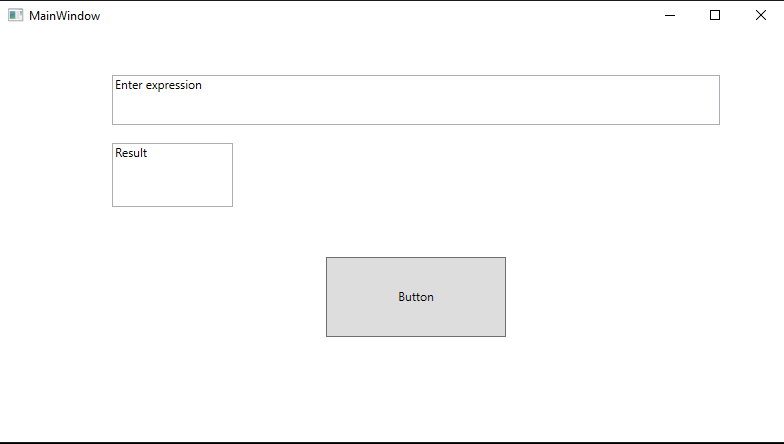
\includegraphics[width=0.9 \columnwidth]{GUI_01}

            \caption{GUI, first revision.}
            \label{gui01}
        \end{center}
    \end{figure}

    \subsection{Testing}
    ERRORS ON T6.BadAssign3, T6.BadCall2 (parameter passing issues), T10.Tan180 (returns 0?)

    \clearpage
% ------------------------------------------------------------- END OF SPRINT ------------------------------------------------------------------
% % ---------------------------------------------------------------- SPRINT 11 ----------------------------------------------------------------
% \section{Sprint 11: Symbol Table as a Class}
% \subsection{Grammar in BNF}
% During this sprint no changes are made to the BNF.

% \subsection{Commentary}
% During this sprint the symbol table was added to a type as a class. Now, member functions of the symbol table handle type checking instead of code written into the match statements.

% \subsection{Testing}
% Refer to Appendix \{X.n\} for unit tests.
% % ------------------------------------------------------------- END OF SPRINT ------------------------------------------------------------------
    \chapter{Final deliverable}\label{Impl}

    Before our final build, we added a number of small features, such as the greater-than-or-equal-to and less-than-or-equal-to operators. Additionally, type-checking for variable assignment was moved to a type as a member function, making our code more maintainable long term.

    \section{Final BNF}
    \begin{verbatim}
Grammar in BNF:

<L>        ::= <R> <Lopt>
<Lopt>     ::= "&&" <R> <Lopt> | "||" <R> <Lopt>
<R>        ::= <E> <Ropt>
<Ropt>     ::=  "<" <E> <Ropt> |
                ">" <E> <Ropt> |
                "<=" <E> <Ropt> |
                ">=" <E> <Ropt> |
                "==" <E> <Ropt>
<E>        ::= <T> <Eopt>
<Eopt>     ::= "+" <T> <Eopt> | "-" <T> <Eopt> | <empty>
<T>        ::= <F> <Topt>
<Topt>     ::= "*" <F> <Topt> | "/" <F> <Topt> |  "%" <F> <Topt> |<empty>
<F>        ::= <NR> <Fopt>
<Fopt>     ::= "^" <NR> <Fopt> | "-" <NR> |<empty>
<NR>       ::=  "!" <NR>
                "Var" <value> "Assign" <NR> |
                "Typ Auto" "Var" <value> "Assign" <NR> |
                "Typ Integer" "Var" <value> "Assign" <NR> |
                "Typ Float" "Var" <value> "Assign" <NR> |
                "Typ Frac" "Var" <value> "Assign" <NR> |
                "Typ Bool" "Var" <value> "Assign" <NR> |
                "Fn" "Var" <value> "Assign" <L> |
                "Var" <value> |
                "Num Int" <value> | "Num Flt" <value> |
                "Num Bool" <value> | "Frac" "Num Frac" <value> |
                "Sin" <NR>  | "Cos" <NR> | "Tan" <NR> |
                "Asin" <NR> | "Acos" <NR> | "Atan" <NR> |
                "LogNat" <NR> | "LogNum" <NR> | "Exp" <NR> |
                "Pi" | "Abs" <NR> |
                "For" "(" "Num Int" <value> ")" "{" <L> "}"
                "(" <L> ")"
    \end{verbatim}
    \section{Final GUI}

    As seen in Figure \ref{gui02}, our application offers both access to our interpreter as well as offering a plotting tool built on top of said interpreter.

    The graphing tool draws a series of plots to the graph by calling the interpreter repeatedly for a series of x values. These plots are made between and upper and lower x bound, determined by the present scale of the graph at the time of plotting. A user specified interval is used by the plotter to determine the change between x values for each plot.

    \begin{figure}[htb]
%\begin{center}
        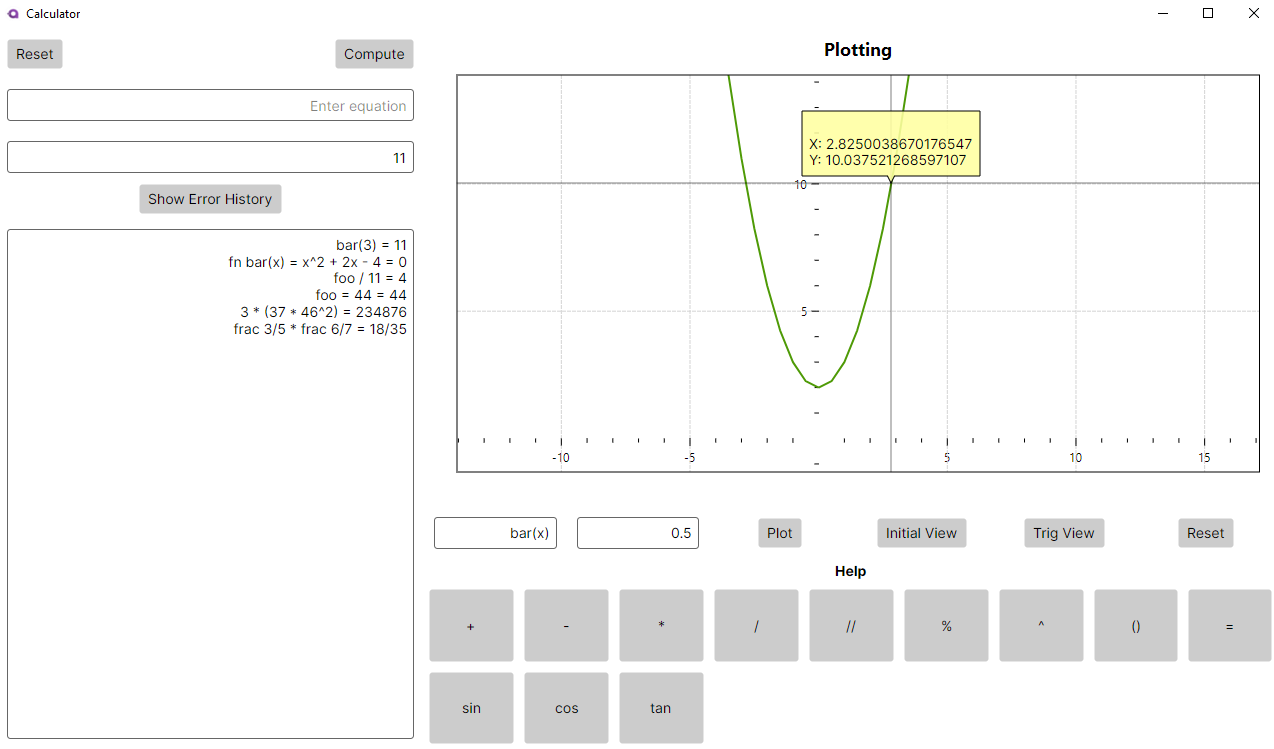
\includegraphics[width=0.9 \columnwidth]{advProgScreencap.png}
        \caption{Final GUI, complete with plotting and computation tools.}
        \label{gui02}
%\end{center}
    \end{figure}

    Because the plotter uses the interpreter to determine which values to plot, it can also draw upon the trigonometric or logarithmic functions defined by the interpreter, as well as any user defined functions. This is seen in Figure \ref{gui02}, where the plotter has plotted bar(x), previously defined in the computation interface as \( x^2 + 2x - 4 \).


    \section{Code architecture}

    Fig.\ \ref{class} shows a UML class diagram (class, sequence and state diagrams are the most frequently used UML diagrams). Illustrating your code architecture - that should be of the MVC family and, considering it is developed in C\# with WPF more specifcally the MVVM pattern - is very important.

    \begin{figure}[htb]
%\begin{center}
        \includegraphics[width=1.0 \columnwidth]{class.png}
        \caption{A UML class diagram to be replaced with yours!}
        \label{class}
%\end{center}
    \end{figure}

    \section{Algorithms}

    Algorithms can be described in this chapter if not already covered in previous sections. Pseudo-code is preferred over code snippets. If you use the latter then make sure it is well commented inside the code or via the figure caption.

    \begin{algorithm}[th]
        \caption{ The Newton-Raphson method }
        \begin{algorithmic}[1]
            \STATE Initialise root based on estimate
            \STATE Set stop criterion
            \\ \texttt{const double error = 0.000001;}
            \WHILE {stop criterion not met}
            \STATE Compute f(root)
            \STATE Compute f'(root)
            \STATE root := root - f(root)/f'(root)
            \ENDWHILE
        \end{algorithmic}
    \end{algorithm}


    Note that code snippets or lists of crucial programming code or large UML diagrams should go in Appendix \ref{app:other} (or further appendices).

    \subsection{Testing}
    The interpreter passed most tests from \ref{ArithTest} through \ref{FinalTest}, with a few exceptions:


    \chapter{Discussion, conclusion and future work}

    Briefly discuss your achievements and put them in perspective with the MoSCoW analysis you specified in Table \ref{Table1}. Also discuss future developments and how you see the deliverable improving if more time could be spent. Note that this section should not be used as a medium to vent frustrations on whatever did not work out (group issues, not enough time, illness, etc.) as this should be dealt with separately - keep it professional!


    \bibliographystyle{apalike}
%\raggedright
    \bibliography{References}


    \appendix
    \chapter{Contributions}
    \section{Contribution Table}
    Here is a table of our contributions. \\

    \begin{table}[h]
        \begin{tabular}{|l|l|l|l|l|}
            \hline
            & Aaron Hurrell & Ethan Colman & Taylor Holton & Connor Stansfield \\ \hline
            Percentage Contributed &               &              &               &                  \\ \hline
        \end{tabular}
    \end{table}

    \section{Aaron Hurrell Contributions}
    \subsection{GUI Contributions}
    I have not contributed to the Graphics User Interface.
    \subsection{Interpreter Contributions}
    \subsection{Report Contributions}

    \section{Ethan Colman Contributions}
    \subsection{GUI Contributions}
    \subsection{Interpreter Contributions}
    \subsection{Report Contributions}

    \section{Taylor Holton Contributions}
    \subsection{GUI Contributions}
    \subsection{Interpreter Contributions}
    \subsection{Report Contributions}

    \section{Connor Stansfield Contributions}
    \subsection{GUI Contributions}
    \subsection{Interpreter Contributions}
    \subsection{Report Contributions}

    State here the \% contribution to the project of each individual member of the group and describe in brief what each member has done (if this corresponds to particular sections in the report then please specify these).

    \chapter{Testing}
    \label{app:test}

% -------------------------------    SPRINT 1 TESTS    ------------------------------
    \section{Arithmetic expression testing}
    \label{ArithTest}
    \begin{tabular}{|p{1.5in}|p{1.5in}|p{1.6in}|p{1.6in}|p{2.4in}|}
        \hline
        TEST NAME       & INPUT                     & EXPECTED RESULT / OUTCOME              & COMMENTS                                \\
        \hline
        T1.Int          & "3"                       & 3                                      &                                         \\
        \hline
        T1.Flt          & "3.5"                     & 3.5                                    &                                         \\
        \hline
        T1.Add          & "1 + 1"                   & 2                                      &                                         \\
        \hline
        T1.Sub          & "2 - 1"                   & 1                                      &                                         \\
        \hline
        T1.Mult         & "2 * 2"                   & 4                                      &                                         \\
        \hline
        T1.DivInt          & "5 / 2"                   & 2                                      &                                         \\
        \hline
        T1.DivFlt          & "5.0 / 2.0"                   & 2.5                                     &                                         \\
        \hline
        T1.Pow          & "2 \^{} 3"                & 8                                      &                                         \\
        \hline
        T1.UnaryPlus    & "+ 3 + 4"                 & 7                                      &                                         \\
        \hline
        T1.UnaryMinus   & "-7 - 3"                   & -10                                    &                                         \\
        \hline
        T1.Brackets     & "(3 + 4)"                 & 7                                      &                                         \\
        \hline
        T1.BIDMAS1      & "3*(3+4)"                 & 21                                     & parentheses precedence                  \\
        \hline
        T1.BIDMAS2      & "3*7\^{}2"                & 147                                    & index precedence                        \\
        \hline
        T1.BIDMAS3      & "6+6/12"                  & 6.5                                    & division precedence over add/sub        \\
        \hline
        T1.BIDMAS4      & "3+2*10"                  & 23                                     & multiplication precedence over add/sub  \\
        \hline
    \end{tabular}
% -------------------------------    SPRINT 2 TESTS    ------------------------------
    \section{Variable Assignment Testing}
    \label{VarAssignTest}
    \begin{tabular}{|p{1.5in}|p{1.5in}|p{1.6in}|p{1.6in}|p{2.4in}|}
        \hline
        TEST NAME       & INPUT                     & EXPECTED RESULT / OUTCOME              & COMMENTS                                \\
        \hline
        T2.BadAssign1   & "= 30"                     & Error                                  &                                         \\
        \hline
        T2.BadAssign2   & "foo ="                   & Error                                  &                                         \\
        \hline
        T2.BadAssign3   & "foo = seventy"           & Error                                  & binding seventy" not in table           \\
        \hline
        T2.AssignNum    & "foo = 3"                 & 3 (Symbol Table should have updated)   &                                         \\
        \hline
        T2.Call         & "foo = 3", "foo"            & 3, 3                                   &                                         \\
        \hline
        T2.InExpression & "foo = 3", "foo + 2"        & 3, 5                                   &                                         \\
        \hline
        T2.VarAsArg     & "foo = 3", "bar = foo", "bar" & "3", "3", "3"                              &                                         \\
        \hline
        T2.Chain        & "foo = bar = 3", "foo", "bar" & "3", "3", "3"                              &                                         \\
        \hline
        T2.Reassign     & "foo = 3", "foo = 2", "foo"   & "3", "2", "2"                               &                                         \\
        \hline
        T2.AssignFloat  & "foo = 3.5"               & 3.5 (Symbol Table should have updated) &                                         \\
        \hline
    \end{tabular}
% -------------------------------    SPRINT 4 TESTS    ------------------------------
    \section{Pi and Absolute Testing}
    \label{PiAbsTest}
    \begin{tabular}{|p{1.5in}|p{1.5in}|p{1.6in}|p{1.6in}|p{2.4in}|}
        \hline
        TEST NAME       & INPUT                     & EXPECTED RESULT / OUTCOME              & COMMENTS                                \\
        \hline
        T4.Pi          & "pi"                                           & 3.141592654                              &                                        \\
        \hline
        T4.AbsNegInt   & "abs -1"                                        & 1                                        &                                        \\
        \hline
        T4.AbsNegFlt   & "abs -1.5"                                      & 1.5                                      &                                        \\
        \hline
        T4.AbsPosInt   & "abs 1"                                         & 1                                        &                                        \\
        \hline
        T4.AbsPosFlt   & "abs 1.5"                                       & 1.5                                      &                                        \\
        \hline
    \end{tabular}
% -------------------------------    SPRINT 5 TESTS    ------------------------------
    \section{Type System Testing}
    \label{TypeSysTest}
    \begin{tabular}{|p{1.5in}|p{1.5in}|p{1.6in}|p{1.6in}|p{2.4in}|}
        \hline
        TEST NAME       & INPUT                     & EXPECTED RESULT / OUTCOME              & COMMENTS                                \\
        \hline
        T5.AutoInt     & "var foo = 1"                                  & 1 (Symbol Table should have Int 1)     &                                        \\
        \hline
        T5.AutoFlt     & "var foo = 1.5"                                & 1.5 (Symbol Table should have Flt 1.5)   &                                        \\
        \hline
        T5.AutoBad     & "var foo = seventy"                            & Error                                    & binding seventy" not in table          \\
        \hline
        T5.IntInt      & "int foo = 1"                                   & 1 (Symbol Table should have Int 1)     &                                        \\
        \hline
        T5.IntFlt      & "int foo = 1.5"                                 & Error                                    & type mismatch                          \\
        \hline
        T5.IntBad      & "int foo = seventy"                             & Error                                    & binding seventy" not in table          \\
        \hline
        T5.FltInt      & "float foo = 1"                                & Error                                    & type mismatch                          \\
        \hline
        T5.FltFlt      & "float foo = 1.5"                              & 1.5 (Symbol Table should have Flt 1.5)   &                                        \\
        \hline
        T5.FltBad      & "float foo = seventy"                          & Error                                    & binding seventy" not in table          \\
        \hline
        T5.ReIntInt    & "int foo = 1", "foo = 2"                          & "1","2"                                   &                                        \\
        \hline
        T5.ReFltFlt    & "float foo = 1.5", "foo = 2.5"                   & "1.5","2.5"                               &                                        \\
        \hline
        T5.ReFltInt    & "float foo = 1.5", "foo = 1"                     & Error                                    & type mismatch                          \\
        \hline
        T5.ReIntFlt    & "int foo = 1", "foo = 1.5"                        & Error                                    & type mismatch                          \\
        \hline
    \end{tabular}
% -------------------------------    SPRINT 6 TESTS    ------------------------------
    \section{Function Assignment Testing}
    \label{FuncAssignTest}
    \begin{tabular}{|p{1.5in}|p{1.5in}|p{1.6in}|p{1.6in}|p{2.4in}|}
        \hline
        TEST NAME       & INPUT                     & EXPECTED RESULT / OUTCOME              & COMMENTS                                \\
        \hline
        \hline
        T6.FuncDec     & "fn foo (x) = x + 3"                           & 0 (Symbol Table should have updated)     & function declaration always returns 0  \\
        \hline
        T6.BadAssign1  & "foo (x) = x + 3"                              & Error                                    &                                        \\
        \hline
        T6.BadAssign2  & "fn (x) = x + 3"                               & Error                                    &                                        \\
        \hline
        T6.BadAssign3  & "fn foo (x) = 3"                               & Error                                    & too many params                        \\
        \hline
        T6.Call        & "fn foo(x) = x + 3", "foo(2)"                    & 0, 5                                     &                                        \\
        \hline
        T6.BadCall1    & "fn foo(x) = x + 3", "foo()"                     & 0, Error                                 &                                        \\
        \hline
        T6.BadCall2    & "fn foo(x) = x + 3", "foo(3 4)"                  & 0, Error                                 & two args                               \\
        \hline
        T6.InExp       & "fn foo(x) = x + 3", "3 + foo(3)"                & 0, 9                                     &                                        \\
        \hline
        T6.Reassign    & "fn foo(x) = x + 3", "fn foo(x) = x + 2", "foo(3)" & 0, 5                                     &                                        \\
        \hline
    \end{tabular}
% -------------------------------    SPRINT 7 TESTS    ------------------------------
    \section{Boolean Testing}
    \label{BoolTest}
    \begin{tabular}{|p{1.5in}|p{1.5in}|p{1.6in}|p{1.6in}|p{2.4in}|}
        \hline
        TEST NAME       & INPUT                     & EXPECTED RESULT / OUTCOME              & COMMENTS                                \\
        \hline
        T7.Assign                         & "foo = true"                            & "true"        &                \\
        \hline
        T7.AssignAuto                     & "var foo = true"                        & "true"        &                \\
        \hline
        T7.AssignBool                     & "bool foo = true"                       & "true"        &                \\
        \hline
        T7.ReBoolBool                     & "foo = true", "foo = false"               & "true", "false" &                \\
        \hline
        T7.ReBoolInt                      & "foo = true "foo = 1"                   & Error         & type mismatch  \\
        \hline
        T7.ReBoolFlt                      & "foo = true "foo = 1.5"                 & Error         & type mismatch  \\
% \hline
% T7.ReBoolFrac                     & "foo = true "foo = frac 3/2"            & Error         & type mismatch  \\
        \hline
        T7.AddInt                         & "true + 3"                              & "4"           &                \\
        \hline
        T7.AddFlt                         & "true + 1.5"                            & "2.5"         &                \\
% \hline
% T7.AddFrac                        & "false + frac 3/2"                      & "3/2"         &                \\
        \hline
        T7.SubInt                         & "false - 3"                             & -3"           &                \\
        \hline
        T7.SubFlt                         & "false - 2.5"                           & -2.5"         &                \\
% \hline
% T7.SubFrac                        & "true - frac 1/2"                       & "1/2"         &                \\
        \hline
        T7.DivInt                         & "true / 2"                              & "0.5"         &                \\
        \hline
        T7.DivFlt                         & "true / 0.8"                            & "1.25"        &                \\
% \hline
% T7.DivFrac                        & "true / frac 1/2"                       & "2/1"         &                \\
        \hline
        T7.MultInt                        & "false * 1"                             & "0"           &                \\
        \hline
        T7.MultFlt                        & "true * 0.7855"                         & "0.7855"      &                \\
% \hline
% T7.MultFrac                       & "true * frac 34/77"                     & "34/77"       &                \\
        \hline
        T7.PowInt                         & "true \^{} 2"                           & "1"        &                \\
        \hline
        T7.PowFlt                         & "false \^{} 0.5"                        & "0"        &                \\
% \hline
% T7.PowFrac                        & "true \^{} frac 1/2"                    & "1 "0"        &                \\
        \hline
        T7.And1                           & "true \&\& true"                            & "true"        &                \\
        \hline
        T7.And2                           & "true \&\& false"                           & "false"       &                \\
        \hline
        T7.And3                           & "false \&\& false"                          & "false"       &                \\
        \hline
        T7.Or1                            & "true \textbar{}\textbar{} true"        & "true"        &                \\
        \hline
        T7.Or2                            & "true \textbar{}\textbar{} false"       & "true"        &                \\
        \hline
        T7.Or3                            & "false \textbar{}\textbar{} false"      & "false"       &                \\
        \hline
        T7.Not                            & "!true"                                 & "false"       &                \\
        \hline
        T7.Equals1                        & "9 = = 9"                                & "true"        &                \\
        \hline
        T7.Equals2                        & "9 = = 8"                                & "false"       &                \\
        \hline
        T7.Less1                          & "$9 < 10$"                                 & "true"        &                \\
        \hline
        T7.Less2                          & "$10 < 9$"                                 & "false"       &                \\
        \hline
        T7.Less3                          & "$9 < 9$"                                  & "false"       &                \\
        \hline
        T7.Greater1                       & "$10 > 9$"                                 & "true"        &                \\
        \hline
        T7.Greater2                       & "$9 > 10$"                                 & "false"       &                \\
        \hline
        T7.Greater3                       & "$9 > 9$"                                  & "false"       &                \\
        \hline
    \end{tabular}
% -------------------------------    SPRINT 8 TESTS    ------------------------------
    \section{Count Controlled Loop Testing}
    \label{LoopTest}
    \begin{tabular}{|p{1.5in}|p{1.5in}|p{1.6in}|p{1.6in}|p{2.4in}|}
        \hline
        TEST NAME       & INPUT                     & EXPECTED RESULT / OUTCOME              & COMMENTS                                \\
        \hline
        T8.NormalUse                     & "foo = 3", "for (3) \{foo = foo + 3\}"   & "3", "12"       &                \\
        \hline
        T8.NonIntCount                   & "foo = 3", "for (0.3) \{foo = foo + 3\}" & Error         &                \\
        \hline
    \end{tabular}
% -------------------------------    SPRINT 9 TESTS    ------------------------------
    \section{Rational Numbers Testing}
    \label{RatNumTest}
    \begin{tabular}{|p{1.5in}|p{1.5in}|p{1.6in}|p{1.6in}|p{2.4in}|}
        \hline
        TEST NAME       & INPUT                     & EXPECTED RESULT / OUTCOME              & COMMENTS                                \\
        \hline
        T9.Rational    & "frac 3/5"                                     & "3/5"                                    &                                        \\
        \hline
        T9.Simplify    & "frac 60/100"                                  & "3/5"                                    &                                        \\
        \hline
        T9.Add         & "frac 30/100 + frac 30/100"                    & "3/5"                                    & = 60/100 = 3/5                         \\
        \hline
        T9.Sub         & "frac 60/100 - frac 30/100"                    & "3/10"                                   & = 30/100 = 3/10                        \\
        \hline
        T9.Div         & "frac 50/100 / frac 2/1"                       & "1/4"                                    & = 25/100 = 1/4                         \\
        \hline
        T9.Mult        & "frac 50/100 * frac 1/2"                       & "1/4"                                    & = 25/100 = 1/4                         \\
        \hline
        T9.Pow         & "frac 3/2 \^{} 2"                              & "9/4"                                    &                                        \\
        \hline
        T9.FracPow     & "frac 9/4 \^{} frac 1/2"                            & "3/2"                                    &                                        \\
        \hline
        T9.AddInt      & "frac 3/2 + 1"                                 & "5/2"                                    &                                        \\
        \hline
        T9.AddFlt      & "frac 3/2 + 0.1234"                       & "16234/10000"                  &                                        \\
        \hline
        T9.SubInt      & "frac 3/2 - 1"                                 & "1/2"                                    &                                        \\
        \hline
        T9.SubFlt      & "frac 3/2 - 0.1234"                       & "6883/5000"                  &                                        \\
        \hline
        T9.DivInt      & "frac 3/2 / 2"                                 & 3/4                                      &                                        \\
        \hline
        T9.DivFlt      & "frac 3/4 / 0.4"                           & "1875/1000"           &                                        \\
        \hline
        T9.MultInt     & "frac 3/2 * 7"                                 & "21/2"                                   &                                        \\
        \hline
        T9.MultFlt     & "frac 3/2 * 0.5"                           & "3/4"                          &                                        \\
        \hline
        T9.AssignFrac1 & "frac foo = frac 3/2"                          & "3/2" (Symbol Table should have updated) &                                        \\
        \hline
        T9.AssignFrac2 & "foo = frac 3/2"                               & "3/2" (Symbol Table should have updated) &                                        \\
        \hline
        T9.AssignFrac3 & "var foo = frac 3/2"                           & "3/2" (Symbol Table should have updated) &                                        \\
        \hline
        T9.ReIntFrac   & "foo = 1", "foo = frac 3/2"                      & "1", Error                                 &                                        \\
        \hline
        T9.ReFltFrac   & "foo = 1.5", "foo = frac 3/2"                    & "1.5", Error                               &                                        \\
        \hline
        T9.ReBoolFrac   & "foo = true", "foo = frac 3/2"                    & "1.5", Error                               &                                        \\
        \hline
        T9.ReFracInt   & "foo = frac 3/2", "foo = 1"                      & "3/2", Error                                 &                                        \\
        \hline
        T9.ReFracFlt   & "foo = frac 3/2", "foo = 1.5"                    & "3/2", Error                               &                                        \\
        \hline
        T9.ReFracBool   & "foo = frac 3/2", "foo = true"                    & "3/2", Error                               &                                        \\
        \hline
        T9.ReFracFrac   & "foo = frac 3/2", "foo = frac 3/4"                    & "3/2", "3/4"                               &                                        \\
        \hline
    \end{tabular}
% -------------------------------    SPRINT 10 TESTS    ------------------------------
    \section{Trigonometric and Logarithmic Function Testing}
    \label{TrigLogTest}
    \begin{tabular}{|p{1.5in}|p{1.5in}|p{1.6in}|p{1.6in}|p{2.4in}|}
        \hline
        TEST NAME       & INPUT                     & EXPECTED RESULT / OUTCOME              & COMMENTS                                \\
        \hline
        T10.Sin90        & "sin 90"                   & 1                                      &                                         \\
        \hline
        T10.Cos0         & "cos 0"                   & 1                                      &                                         \\
        \hline
        T10.Sin0         & "sin 0"                    & 0                                      &                                         \\
        \hline
        T10.Cos90        & "cos 90"                  & 0                                      &                                         \\
        \hline
        T10.Sin45        & "sin 45"                   & 0.7071067812                           &                                         \\
        \hline
        T10.Cos45        & "cos 45"                  & 0.7071067812                           &                                         \\
        \hline
        T10.Tan0         & "tan 0"                   & 0                                      &                                         \\
        \hline
        T10.Tan45        & "tan 45"                  & 1                                      &                                         \\
        \hline
        T10.Tan180       & "tan 180"                 & undefined or Error                     &                                         \\
        \hline
        T10.ASin1        & "asin 1"                   & 90                                     &                                         \\
        \hline
        T10.ACos0        & "acos 0"                   & 90                                     &                                         \\
        \hline
        T10.ASin0        & "asin 0"                   & 0                                      &                                         \\
        \hline
        T10.ACos1        & "acos 1"                   & 0                                      &                                         \\
        \hline
        T10.ASin0.7      & "asin 0.7071067812"        & 45                                     &                                         \\
        \hline
        T10.ACos0.7      & "acos 0.7071067812"        & 45                                     &                                         \\
        \hline
        T10.ATan0        & "atan 0"                   & 0                                      &                                         \\
        \hline
        T10.ATan1        & "atan 1"                   & 45                                     &                                         \\
        \hline
        T10.ATanLarge    & "atan 999"                 & 89.94264689                            & as x increases atan x approaches 180    \\
        \hline
        T10.ASinRange1   & "asin 2"                   & Error                                  &                                         \\
        \hline
        T10.ASinRange2   & "asin -2"                  & Error                                  &                                         \\
        \hline
        T10.ACosRange1   & "acos 2"                   & Error                                  &                                         \\
        \hline
        T10.ACosRange2   & "acos -2"                  & Error                                  &                                         \\
        \hline
        T10.LnE          & "ln 2.71828182846"        & 1                                      & as x increases atan x approaches 180    \\
        \hline
        T10.Ln0          & "ln 0"                    & undefined or Error                     &                                         \\
        \hline
        T10.LogX\_Y      & "log 2 8"                 & 3                                      &                                         \\
        \hline
        T10.LogX\_X      & "log 2 2"                 & 1                                      &                                         \\
        \hline
        T10.Log0         & "log 2 0"                 & undefined or Error                     &                                         \\
        \hline
        T10.Exp          & "e\^{}1"                   & 2.718281828                            &                                         \\
        \hline
    \end{tabular}
% ------------------------------    FINAL SPRINT TESTS    -----------------------------
    \section{Final Sprint Additional Testing}
    \label{FinalTest}
    \begin{tabular}{|p{1.5in}|p{1.5in}|p{1.6in}|p{1.6in}|p{2.4in}|}
        \hline
        TEST NAME       & INPUT                     & EXPECTED RESULT / OUTCOME              & COMMENTS                                \\
        \hline
        F.LessEq1                         & $"9 <= 10"$                                & "true"        &                \\
        \hline
        F.LessEq2                         & $"10 <= 9"$                                & "false"       &                \\
        \hline
        F.LessEq3                         & $"9 <= 9"$                                 & "true"        &                \\
        \hline
        F.GreaterEq1                      & $"10 >= 9"$                                & "true"        &                \\
        \hline
        F.GreaterEq2                      & $"9 >= 10"$                                & "false"       &                \\
        \hline
        F.GreaterEq3                      & $"9 >= 9"$                                 & "true"        &                \\
        \hline
    \end{tabular}
% -------------------------------------------------------------------------------------
    \section{MoSCoW Requirements Analysis} \label{MOSCOW}
    \begin{center}
        \begin{tabular}{|p{1in}|p{2in}|p{2.5in}|} \hline
        Priority & Task & Comments \\ \hline \hline

% MUST
        \multirow{3}{1in}{Must}
        & Expressions (INT1) & Outline basic operator precedence structure and implement simple binary operations (+, -, /, *, \verb|^|) as well as unary (+ / -) operators. \\ \cline{2-3}
        & Assignment (INT2) & Allow for simple variable assignment by assigning user values to a table, associated with a user defined identifier. \\ \cline{2-3}
        & GUI (GUI1) & Provide a graphical interface capable of taking user input, processing it via the interpreter, and displaying the results. \\ \cline{2-3}
        & Plotting (GUI2) & Expand the graphical interface to allow for graph plotting. \\ \cline{2-3}
        & Numbers as Floats/Ints & Related to INT1 and mandatory \\ \hline \hline

% SHOULD
        \multirow{3}{1in}{Should}
        & Rational Numbers & Add support for rational numbers, represented internally as a pair of numbers (numerator and denominator). \\ \cline{2-3}
        & Complex Numbers & Add support for complex numbers, represented internally as a pair of numbers (real and imaginary components).  \\ \cline{2-3}
        & Functions & Expand symbol table used for variable assignment to allow for user defined functions, including functions to parse and replace parameters where appropriate.  \\ \cline{2-3}
        & Booleans & Add support for boolean values, as well as both logical (\verb|&&| or \textbar{}\textbar{}) and relational (\verb|<|, \verb|>| and \verb|==|) operators.   \\ \cline{2-3}
        & Static Type System & Assign specific types to numbers, and conduct type checking whenever a user assigns a value to a variable or function. \\ \hline \hline
        \end{tabular}
    \end{center}
    \begin{center}
        \begin{tabular}{|p{1in}|p{2in}|p{2.5in}|} \hline
        Priority & Task & Comments \\ \hline \hline
% COULD
        \multirow{3}{1in}{Could}
        & Iteration and Control Flow (INT3) & Add functionality to either the plotter or interpreter allowing a user to define a function to plot, as well as a range to plot over and an interval to define how frequently to plot. Plotter should produce a graph representing this series of plots. \\ \cline{2-3}
        & Condition Control (Assumes boolean implementation) & Add if/else statements to the interpreter, allowing the user to define more complex branching functions. \\ \cline{2-3}
        & Math Tools (INT4) & Add support for more complex mathematics, such as calculus and root finding via methods such as Newton-Raphson approximation.\\ \cline{2-3}
        & Expanded GUI Features (GUI3) (Assumes INT4 implementation) & Expand our GUI to support features introduced in Math Tools (INT4), such as drawing tangent lines utilising differentiation support introduced in INT4.\\\hline \hline

% SHOULD NOT
        \multirow{3}{1in}{Should not}
        & Compiler (INT5) & Amend interpreter to instead compile to machine code or some intermediate language (such as C). \\ \cline{2-3}
        & Compiler Interface (GUI4) (Assumes INT5 implementation) & Add a field to GUI allowing users to enter uncompiled code and another field to access compiled code. \\ \hline
        \end{tabular}
    \end{center}
% -------------------------------------------------------------------------------------

    \chapter{Images}
    \section{Wolfram Alpha Images:Plotted} \label{WolframPlotted}

    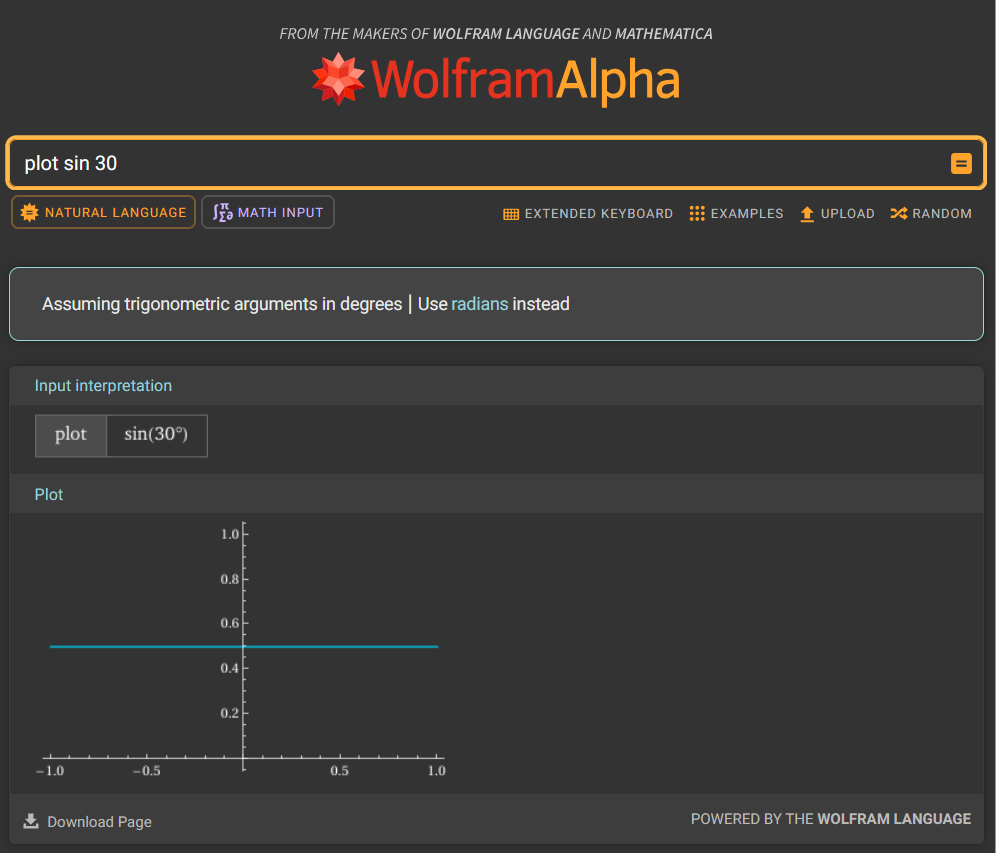
\includegraphics[width=160mm]{Screenshot 2025-01-03 161746.png} \\


    \section{Wolfram Alpha Images:Non-Plotted}\label{WolframUnplotted}

    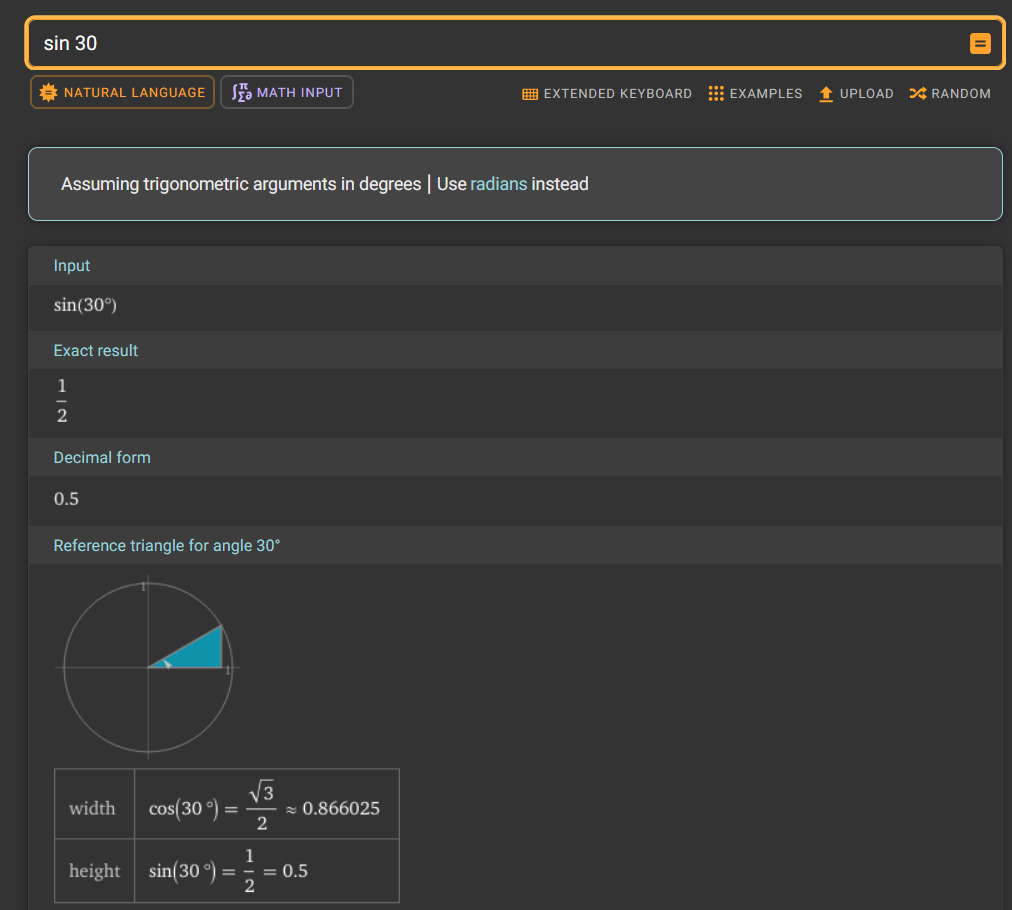
\includegraphics[width = 160mm]{Screenshot 2025-01-03 162013.png} \\

    \label{app:other}
\end{document}

& ====================================================================================
& ====================================================================================

% \clearpage
% \begin{table}[h]
% \caption{Arithmetic expression tests. Note that floating pointing values are accurate to three decimal places for the fractional part. ResE is expected result and ResA is actual result. \\}
% \begin{tabular}{|p{1.8in}|p{0.5in}|p{0.6in}|p{0.6in}|p{1.4in}|} \hline
% Expression & ResE & ResA& Pass/Fail & Action/comment \\ \hline \hline
% $5*3+(2*3-2)/2+6$ & 23 & 23 & Pass &  ... \\ \hline
% $9-3-2$ & 4 & 4& Pass & left assoc.\  \\ \hline
% $10/3$ & 3 & 3& Pass & int division  \\ \hline
% $10/3.0$ & 3.333 & 3.3333333& Pass & float division \\ \hline
% $10\%3$ & 1 & 1& Pass & \\ \hline
% $10 - -2$ & 12 & 12& Pass & unary minus\\ \hline
% $-2 + 10$ & 8 & 8& Pass & \\ \hline
% $3*5\verb|^|(-1+3)-2\verb|^|2*-3$ & 87 & 87& Pass & power test \\ \hline
% $-3\verb|^|2$ & -9(*) or 9 & 9& Pass & precedence \\ \hline
% $-7\%3$ & 2(*) or -1 & -1& Pass & precedence (*)Python\\ \hline
% $2*3^2$ & 18 & 18& Pass & precedence pow > mult \\ \hline
% $3*5\verb|^|(-1+3)-2\verb|^|-2*-3$ & 75.750 or 75 & 75& Pass & \\ \hline
% $3*5\verb|^|(-1+3)-2.0\verb|^|-2*-3$ & 75.750 &75.75 & Pass & \\ \hline
% $(((3*2--2)))$ & 8 & 8& Pass & \\ \hline
% $(((3*2--2))$ & Error &Error & Pass & syntax error \\ \hline
% $-((3*5-2*3))$ & -9 & -9& Pass &  minus expression \\ \hline
% $x = 3; (2*x)-x\verb|^|2*5$ & -39 & -39& Pass & var assign \\ \hline
% $x = 3; (2*x)-x\verb|^|2*5/2$ & -16 & -16 & Pass & \\ \hline
% $x = 3; (2*x)-x\verb|^|2*(5/2)$ & -12 &  -12 & Pass & \\ \hline
% $x = 3; (2*x)-x\verb|^|2*5/2.0$ & -16.5 & -16.5 & Pass & \\ \hline
% $x = 3; (2*x)-x\verb|^|2*5\%2$ & 5 & 5 & Pass &  \\ \hline
% $x = 3; (2*x)-x\verb|^|2*(5\%2)$ & -3 &  -3 & Pass &  \\ \hline
% ... & ... & ... & ... & ... \\ \hline
% \end{tabular}
% \label{Table2}
% \end{table}

% \section{GUI testing}\label{GUITest}

% \section{Plotting testing}\label{PlotTest}
% \section{Variable Assignment Testing}\label{VarAssTest}
% % \usepackage{hhline}


% \begin{table}[h]
% \centering
% \caption{Variable Assignment tests. Note that floating pointing values are accurate to three decimal places for the fractional part. ResE is expected result and ResA is actual result. \\}
% \label{Table2}
% \begin{tabular}{|p{1.8in}|p{0.5in}|p{0.6in}|p{0.6in}|p{1.4in}|}
% \hline
% Expression                          & ResE  & ResA & Pass/Fail & Action/comment  \\
% \hline \hline
% $int x = 10; x$                     & 10    &      &           &                 \\
% \hline
% $int x = 1; int five = 1; x + five$ & 2     &      &           &                 \\
% \hline
% $float n = 10.2; n = 10;n$          & 10.0  &      &           &                 \\
% \hline
% $float y = 1.2; float y = 1.3;y$    & Error &      &           &                 \\
% \hline
% \$\$                                &       &      &           &                 \\
% \hline
% \$\$                                &       &      &           &                 \\
% \hline
% \$\$                                &       &      &           &                 \\
% \hline
% \end{tabular}
% \end{table}


% \section{Trigonometric and Logarithmic Function Testing}\label{TrigTest}

% \begin{table}[h]
% \centering
% \caption{Trigonometric and Logarithmic Function Tests. Note that floating pointing values are accurate to three decimal places for the fractional part. ResE is expected result and ResA is actual result. \\}
% \label{Table3}
% \begin{tabular}{|l|l|l|l|l|}
% \hline
% Expression                  & ResE                            & ResA & Pass/Fail & Action/comment  \\
% \hline \hline
% $sin 30$                    & 0.5                             &      &           &                 \\
% \hline
% $sin 270$                   & -1                              &      &           &                 \\
% \hline
% $sin -20$                   & -0.3420201433                   &      &           &                 \\
% \hline
% $sin 2000$                  & -0.342020143                    &      &           &                 \\
% \hline
% $sin two$                 & error                           &      &           &                 \\
% \hline
% $int two = 30; sin two$   & 0.5                             &      &           &                 \\
% \hline
% $cos 60$                  & 0.5                             &      &           &                 \\
% \hline
% $cos 360$                 & 1                               &      &           &                 \\
% \hline
% $cos -80$                 & 0.1736481777                    &      &           &                 \\
% \hline
% $cos -1920$               & -0.5                            &      &           &                 \\
% \hline
% $cos cosine$              & error                           &      &           &                 \\
% \hline
% $int two = 60; cos two$   & 0.5                             &      &           &                 \\
% \hline
% $tan 90$                  & Error-\textgreater{} undefined  &      &           &                 \\
% \hline
% $tan 180$                 & 0                               &      &           &                 \\
% \hline
% $tan -300$                & 1.732050808                     &      &           &                 \\
% \hline
% $tan tany$                & error                           &      &           &                 \\
% \hline
% $int two = 180; tan two$  & 0                               &      &           &                 \\
% \hline
% $asin 0.5$                & 30                              &      &           &                 \\
% \hline
% $asin -1$                 & -90                             &      &           &                 \\
% \hline
% $asin -0.3420201433$      & 20                              &      &           &                 \\
% \hline
% $asin test$               & error                           &      &           &                 \\
% \hline
% $int two = 0.5; asin two$ & 30                              &      &           &                 \\
% \hline
% $asin 1.5$                & Error -\textgreater{} undefined &      &           &                 \\
% \hline
% $asin -1.5$               & Error - undefined               &      &           &                 \\
% \hline
% $acos 0.5$                & 60                              &      &           &                 \\
% \hline
% $acos -1$                 & 180                             &      &           &                 \\
% \hline
% $acos 0.1736481777$       & 80                              &      &           &                 \\
% \hline
% $acos test$               & Error                           &      &           &                 \\
% \hline
% $int two = 0.5; acos two$ & 60                              &      &           &                 \\
% \hline
% $acos 1.5$                & Error - undefined               &      &           &                 \\
% \hline
% $acos -1.5$               & Error - undefined               &      &           &                 \\
% \hline
% $ atan 1$                 & 45                              &      &           &                 \\
% \hline
% $ atan 0.3$               & 16.69924423                     &      &           &                 \\
% \hline
% $ atan 01.732050808$      & 60                              &      &           &                 \\
% \hline
% $ atan test$              & Error                           &      &           &                 \\
% \hline
% $int two = 0.5; atan two$ & 26.56505118                     &      &           &                 \\
% \hline
% $ atan 1.5$               & 56.30993247                     &      &           &                 \\
% \hline
% $ logNat 1$               & 0                               &      &           &                 \\
% \hline
% $ logNat 20$              & 2.995732274                     &      &           &                 \\
% \hline
% $ logNat 359$             & 5.883322388                     &      &           &                 \\
% \hline
% $ logNat -1$              & Error - undefined               &      &           &                 \\
% \hline
% $ logNum 10 100$          & 2                               &      &           &                 \\
% \hline
% $ logNum -2 10$           & Error                           &      &           &                 \\
% \hline
% $ logNum 2 -4$            & Error                           &      &           &                 \\
% \hline
% \end{tabular}
% \end{table}

% \section{Functions Testing}\label{FuncTest}
% \section{Pi and Abs Testing}\label{PiTest}

% \begin{table}[h]
% \centering
% \caption{Pi and Abs Tests. Note that floating pointing values are accurate to three decimal places for the fractional part. ResE is expected result and ResA is actual result. \\}
% \label{Table4}
% \begin{tabular}{|l|l|l|l|l|}
% \hline
% Expression       & ResE        & ResA & Pass/Fail & Action/comment  \\
% \hline \hline
% $pi$             & 3.141592654 &      &           &                 \\
% \hline
% $2*pi$           & 6.283185307 &      &           &                 \\
% \hline
% $pi^2$           & 9.869604401 &      &           &                 \\
% \hline
% $int pi = pi;pi$ & Error       &      &           &                 \\
% \hline
% $ abs -2.5 $   & 2.5         &      &           &                 \\
% \hline
% $ abs 2.5 $    & 2.5         &      &           &                 \\
% \hline
% $ abs text $   & Error       &      &           &                 \\
% \hline
% \end{tabular}
% \end{table}

% \section{Static Type System Testing}\label{StaticTest}
% \section{Rational Number Testing}\label{RationTest}
% \section{Boolean Testing}\label{BoolTest}

% \begin{table}
% \centering
% \caption{Boolean Tests. Note that floating pointing values are accurate to three decimal places for the fractional part. ResE is expected result and ResA is actual result. \\}
% \label{Table5}
% \begin{tabular}{|l|l|l|l|l|}
% \hline
% Expression       & ResE  & ResA & Pass/Fail & Action/comment  \\
% \hline \hline
% $true$           & true  &      &           &                 \\
% \hline
% $false$          & false &      &           &                 \\
% \hline
% $!true$          & false &      &           &                 \\
% \hline
% $!false$         & true  &      &           &                 \\
% \hline
% $ !!true $     & true  &      &           &                 \\
% \hline
% $12$           & true  &      &           &                 \\
% \hline
% $ -1020 $      & true  &      &           &                 \\
% \hline
% $45<21$          & false &      &           &                 \\
% \hline
% $23 < -12$       & false &      &           &                 \\
% \hline
% $2>1$            & true  &      &           &                 \\
% \hline
% $20>-10$         & true  &      &           &                 \\
% \hline
% $21>45$          & false &      &           &                 \\
% \hline
% $-12>23$         & false &      &           &                 \\
% \hline
% $2<=2$           & true  &      &           &                 \\
% \hline
% $2<=3$           & true  &      &           &                 \\
% \hline
% $2=<3$           & Error &      &           &                 \\
% \hline
% $102 <= 100$     & false &      &           &                 \\
% \hline
% $102 >= 102$     & true  &      &           &                 \\
% \hline
% $98 >= 105$      & false &      &           &                 \\
% \hline
% $7 == 7$         & true  &      &           &                 \\
% \hline
% $67 == 21$       & false &      &           &                 \\
% \hline
% $21<34 == 45>1$  & true  &      &           &                 \\
% \hline
% $true || true$   & true  &      &           &                 \\
% \hline
% $true || false$  & true  &      &           &                 \\
% \hline
% $false || false$ & false &      &           &                 \\
% \hline
% $true \&\& false$  & false &      &           &                 \\
% \hline
% $false \&\& false$ & false &      &           &                 \\
% \hline
% $true \&\& true$   & true  &      &           &                 \\
% \hline
% ...              & ...   & ...  & ...       & ...             \\
% \hline
% \end{tabular}
% \end{table}